\section{BON extraction}
Section \ref{design-bon-extraction} described how the textual \textsc{bon} extraction tool consists of two parts: an internal representation of textual \textsc{bon} and an interface to the Eiffel part of EiffelStudio. This section will describe the structure of these two, and how they are implemented.
\subsection{The Interface to EiffelStudio	}
\label{why_interface_takes_care_of_formal_and_informal}
As mentioned above, to create a view in EiffelStudio it is needed to redefine certain classes. First and foremost is the class text formatter. The main feature to note in this is the \textit{generate\textunderscore text} feature that is called by the format feature in the same class, which is invoked from the development window class. This calls a feature inherited from a \textsc{textual$\textunderscore$bon$\textunderscore$format$\textunderscore$table} called either \textit{informal$\textunderscore$bon$\textunderscore$context$\textunderscore$text} or \textit{formal$\textunderscore$bon$\textunderscore$context$\textunderscore$text}, depending on the dynamic type of the formatter. Which dynamic type is being used decides what kind of textual \textsc{bon} is being extracted. This feature from a shared format table sets a \textit{is$\textunderscore$informal$\textunderscore$bon} or \textit{is$\textunderscore$formal$\textunderscore$bon} flag depending on the context. This flag is passed on by the \textsc{class$\_$text$\_$formatter} to the \textsc{text$\_$formatter$\_$decorator} which uses the information to create the appropriate \textsc{ast$\_$decorated$\_$output$\_$strategy}.
\begin{figure}
\centerline{
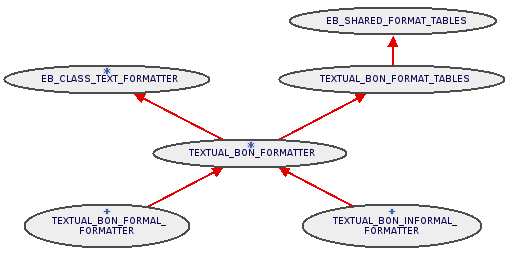
\includegraphics[scale=0.7]{images/textual-bon-formatter.png}
}
\caption{\textsc{textual$\textunderscore$bon$\textunderscore$formatter} inheritance relations.}
\label{fig:textual_bon_formatter}
\end{figure}

\begin{figure}[h]
\centerline{
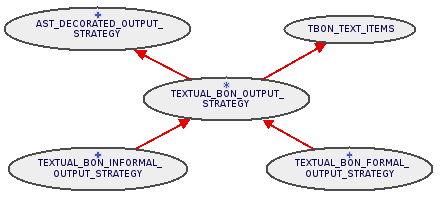
\includegraphics[scale=0.7]{images/bon-extraction-output-strategy.png}
}
\caption{\textsc{textual$\textunderscore$bon$\textunderscore$output$\textunderscore$strategy} inheritance relations.}
\label{fig:bon-extraction-output-strategy}
\end{figure}

\paragraph{}
The output strategies inherits a feature called \textit{process$\_$class$\_$as}. The purpose of this feature is to generate the desired output from a \textsc{class$\_$as}, which is the abstract eiffel syntax representation of a class. In the implementation of the \textsc{bon} tool, this is done by instantiating the previously mentioned meta-object (See figure \ref{fig:bon_extraction_3} on page \pageref{fig:bon_extraction_3}) from the \textsc{class$\_$as} object, which then generates the internal representation. This mechanism will be explained in detail in section \ref{tbon_class}.

\paragraph{}
To keep the \textsc{bon} formatters and output strategies both similar, yet distinct at the same time, they both inherit from a shared deferred class, as it can be seen in figures \ref{fig:textual_bon_formatter} and \ref{fig:bon-extraction-output-strategy}. This gives them a polymorphic characteristic, which makes handling these classes easier as it is not always needed know whether you are in formal or informal context at a given point in time. This is not utilized by this project, but is done to make future development more seamless. 

\subsection{The Internal BON Representation}
\begin{figure}[H]
\centerline{
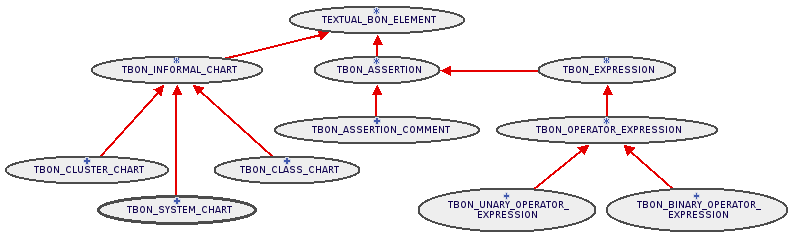
\includegraphics[scale=0.7]{images/bon-extractor-mog-overview.png}
}
\caption{An excerpt of the classes created for the internal representation of textual \bon{} in EiffelStudio.}
\label{fig:textual_bon_formatter}
\end{figure}
A series of classes has been created to represent the elements of the \bon{} grammar in \cite{walden1995}. Each of these classes store the information required about the represented grammar element in order to be able to generate textual \bon{}. The presence of mandatory elements of the grammar, such as a class name in a class chart, is ensured through the use of  \textit{attached} features\footnote{In the world of Eiffel, the \textit{attached} keyword ensures that a reference cannot be \textit{Void}. Thus, it must refer to an object.} and contracts (invariants and pre- and postconditions). A class represent a grammar element knows how to process itself, and itself only. If it contains other elements, such as a class containing features, the class will have a collection of features, and then delegate the processing of features to the class representing features. Any nested relations are processed this way.

\paragraph{}
This representation of textual \textsc{bon} is based around the \textsc{textual$\_$bon$\_$element} class. From this class, all classes inherit the features \textit{process$\_$to$\_$formal$\_$textual$\_$bon} and  \textit{process$\_$to$\_\newline$informal$\_$textual$\_$bon}. These features format textual \textsc{bon} based on the metadata in the enclosing class. For elements that only exist in either formal or informal \bon{} or have identical representations in the two, these two features have been renamed and joined into the same feature (\textit{process$\_$to$\_$textual$\_$bon}).

\subsubsection{Completeness}
To give a feeling of working with complete textual \bon{}, other parts than merely the class chart or the class component for the current class is generated. In the informal textual \bon{ } view both a system chart and cluster chart are created. A system chart keeps track of its contained cluster through a collection of clusters, and a cluster chart has a collection of clusters and classes. When a system chart is asked to process itself, it will also invoke the processing feature of its contained clusters, which then does the same for its contained classes and clusters. All other objects in the \bon{} representation handle processing in the same way. Analogous to the generation of a system chart and a cluster chart in the extraction of informal \bon{}, a cluster component is generated when extraction formal \bon{}.

\subsubsection{Indexing}
In order to translate the semantics of the indexing clause in Eiffel properly to informal textual \bon{} a few alterations are made to it. Certain indexing tag names are identified as explanations and removed from the indexing clause and processed under the \textit{explanation} keyword of class charts in informal textual \bon{}. In the current implementation, the tags identified are \textit{description} and \textit{explanation} (the idenficiation is not case-sensitive). This is identified by the feature \textit{is$\_$explanation$\_$string} in \textsc{tbon$\_$class$\_$chart}. Furthermore an extra entry into the indexing clause of a class chart is added to the informal textual \bon{}. To identify which cluster a class belongs to, a \textit{belongs$\_$to} tag has been added. This is not strictly necessary in this implementation, as one cluster is only ever made. However, if this was to be expanded to scale to a full system, one might want multiple clusters. As such, this tag provides the reader of the specification with a better overview.

\subsubsection{Inheritance}
To create an overview from the point of view of the current class, a specification for all descendants of the current class is also extracted. This is done by inspecting the \textit{direct$\_$descendants} feature of the compiled class object from EiffelStudio (\textsc{class$\_$c}). These classes are then added to the cluster, and then processed into textual \bon{}.

\subsubsection{The meta-object}
\label{tbon_class}
When the output strategy receives the abstract Eiffel syntax, the internal \bon{} representation is created. As previously mentioned, this is done through a meta object. This object is called \textsc{tbon$\_$class}. \textsc{tbon$\_$class} takes a \textsc{class$\_$as} object and instantiates the internal representation of the \bon{}. It does this by inspecting the abstract syntax of the class and giving the needed information to the textual \bon{} objects.